\subsection{Two exact algorithms for certifying a submitted solution}\label{app:td-native}

A fast exact checker can exploit the fact that each vehicle clock is nondecreasing. We compare 2 algorithms on the same binary64 operands. Both convert each operand to its exact rational value, use inclusive deadlines and return the minimum duration and the earliest departure attaining it. The C++ implementations share the same GMP rational knots, interval slopes and Python binding. The \href{https://gmplib.org/manual/Rational-Conversions}{GMP conversion from binary64} is exact.

\paragraph{Compose the route prefix.}
After each visit, keep the arrival or ready time as a piecewise-affine function of the initial departure. To append an arc, scan the prefix and arc knots in time order. Where an increasing prefix segment crosses an arc knot, insert its exact preimage into the new prefix. At a jump, keep the attained ordinate and the right limit separately. If the prefix stays constant at an arc knot, the vehicle attains the lower ordinate throughout that plateau. Waiting can add a breakpoint, and a deadline can truncate the feasible interval. Finally compare return time minus departure at the attained breakpoints in increasing departure order. For continuous FIFO functions, Visser and Spliet give a linear-time scan for each composition. Here the scan also carries the two ordinates at a jump. \href{https://repub.eur.nl/pub/100852/EI2017-23.pdf}{Visser and Spliet, Section~3}.

\paragraph{Sweep through departures.}
Evaluate the lowest allowed departure first. If it is infeasible, FIFO and the closed upper bounds exclude all later departures. Otherwise trace the vehicle's clock through the route. Just to the right of that departure, the clock at each visit has an exact value and rate of increase. A positive rate determines when it will next meet an arc knot, waiting threshold or deadline. A zero rate at a knot keeps the vehicle on its attained branch. The first event across the visits ends an interval on which route duration is affine. Left continuity gives the attained return at its right endpoint. Repeating this operation visits the candidates for the minimum without constructing every prefix function. Both algorithms test singleton domains and keep the earliest departure on a tie.

\begin{table}[htbp]
\centering
\small
\begin{tabular}{@{}lrr@{}}
\toprule
Evaluator & Including preparation (ms) & Prepared (ms)\\
\midrule
Python exact partitioning reference & 30.217 & \\
Python exact departure sweep & 1.794 & 1.065\\
C++/GMP exact prefix composition & 0.234 & 0.134\\
C++/GMP exact departure sweep & 0.236 & 0.125\\
Python v0.12 released fold & & 0.063\\
\bottomrule
\end{tabular}
\caption{Grid'5000 timings on the same 24 routes as Table~\ref{tab:td-matched-runtime}. Entries are median milliseconds per route. Blank cells indicate unmeasured scopes. The released fold returns its historical binary64 result.}\label{tab:td-native-route}
\end{table}

We ran 2 fresh serial processes on the Nancy Grid'5000 cluster, pinned to 1 logical CPU of a Xeon Gold 5220, using CPython 3.13.12, GCC 14.2 and GMP 6.3. For each route and method, each process warms the call and times 3 calibrated batches. We take the median within each process, then the median across processes, then across routes. In the preparation-inclusive scope the new algorithms start with the binary64 operands gathered for the route. The original partitioning reference also rebuilds its arc lookup from the loaded record. In the prepared scope the arc representations are already in memory. Both native scopes include transferring the exact result to Python. The median paired speedup over the partitioning reference is $107.3$ for native composition including preparation. On the Grid'5000 node, prepared native composition takes $1.84$ times the v0.12 route time by the same paired comparison. Repeating the matched comparison on an i7-12700H gave a median paired speedup of $144.6$ for preparation-inclusive native composition over the Python partitioning reference.

For a submitted solution the checker starts with the instance fields and an index of its materialized binary64 arcs. It checks route coverage, fleet size and capacities, gathers and prepares each route, optimizes its departure and sums the exact durations and any vehicle charge. File loading, family materialization and result serialization are outside this timer. Both native algorithms reproduce the independent partitioning reference's exact durations and earliest departures for all 1,141 routes. The resulting median time for a complete solution is 1.36~ms for composition and 1.35~ms for the sweep on the 146 Dabia2013 solutions. On the 35 broader solutions the medians are 18.35~ms for composition and 14.26~ms for the sweep (Figure~\ref{fig:td-native-solution}).

\begin{figure}[htbp]
\centering
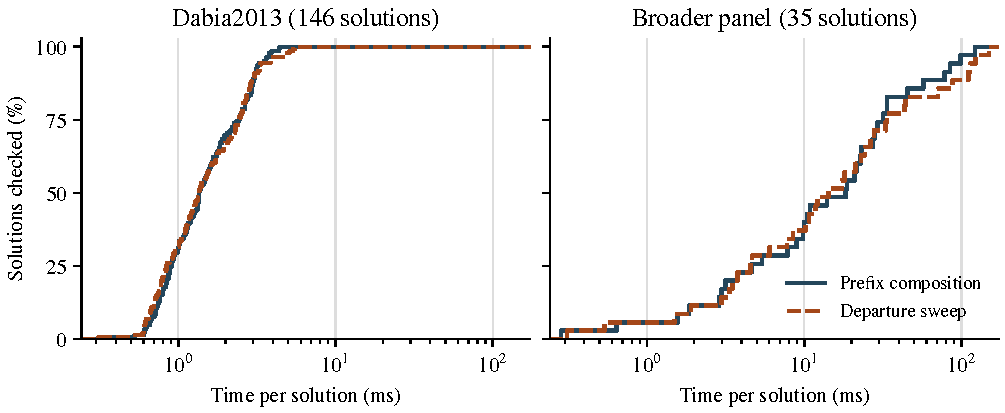
\includegraphics[width=0.92\linewidth]{figures/td-fixed-solution-time.pdf}
\caption{Fraction of submitted solutions checked within a given time, including route preparation, exact scheduling and objective aggregation. Each point is the median for one instance and candidate. The horizontal scale is logarithmic. Times are from the Grid'5000 node.}\label{fig:td-native-solution}
\end{figure}

In a separate scale check on the i7-12700H we selected one available solution per family at its largest available customer count, resolving ties by record identifier. On the 2 selected 1,000-customer solutions, native composition checked 91 Lera2026 routes in 79~ms and 66 Poryos2026 routes in 465~ms. The departure sweep took 89 and 779~ms respectively. These cases illustrate the effect of route structure and arc complexity at the same customer count.

\paragraph{Starting from an instance file.}
We timed the released v0.12 loader followed by the native composition checker on 3 published route sets. These cases exercise a stored ATF, reconstruction from a road graph and traffic overlay, and reconstruction from an IGP speed profile. The loader reads the descriptor and candidate and verifies the materialized ATF identity. The checker builds its model, validates the solution and computes the exact objective and departures. The last step writes the exact result to a JSON buffer. Each case ran in 5 fresh processes on the Grid'5000 node with a warm filesystem cache. We verified the result with the departure sweep after each run.

\begin{table}[htbp]
\centering
\small
\begin{tabular}{@{}lrrrr@{}}
\toprule
Instance & Customers & Load (ms) & Check (ms) & Total (ms)\\
\midrule
Blauth-Nairobi, stored & 10 & 3.02 & 0.67 & 3.98\\
Poryos-Lyon, road graph & 10 & 437.59 & 3.74 & 441.95\\
Lera C1\_2\_1 S1, IGP & 200 & 926.08 & 26.62 & 953.24\\
\bottomrule
\end{tabular}
\caption{Median times from input files to a serialized exact result using the released loader and prototype checker. Each column is a separate median. The total includes result serialization.}\label{tab:td-native-loader}
\end{table}

For the 200-customer Lera case the loader reconstructs and verifies 40,200 directed ATFs before checking the submitted routes. For repeated submissions to the same instance, retaining the verified materialization in memory can therefore save more time than changing the route algorithm.

\paragraph{What exact solution records have to store.}
Both native algorithms agreed on feasibility, duration and earliest departure for all 61,500 routes on the 3,052 available incumbent records. An independent exact forward traversal replayed every departure and recovered all route durations and solution objectives. The 20 records with unavailable materialization files remain outside this comparison. The released solution total matched the once-rounded exact objective on 1,300 records under v0.11 and 1,565 under v0.12. Equality of the released value with the unrounded rational objective held on 454 and 624 records, respectively.

Even when every stored operand is binary64, TD interpolation and boundary preimages can introduce non-dyadic denominators. Summing routes can give a much longer denominator than any individual route requires. Across the store, the largest integer in an exact route duration or departure had 1,093 decimal digits. For 358 solution totals, the reduced numerator or denominator exceeded 4,300 digits, the \href{https://docs.python.org/3.13/library/stdtypes.html#integer-string-conversion-length-limitation}{default threshold for ordinary decimal integer conversions in CPython}. One 1,000-customer Poryos-Lyon solution had a numerator of 10,405 digits. An implementation of Section~\ref{sec:results} must preserve every digit of these strings. All 3,052 exact objectives round-tripped as canonical decimal strings on the Grid'5000 node. The largest numerator and denominator together occupied 20,837 bytes in their compact JSON record. This encoding test is separate from scheduling.
